\documentclass[11pt]{article}
\usepackage[textwidth=18.0cm, textheight=23.0cm, top=2.0cm]{geometry}
\usepackage{pst-all}
\usepackage{amssymb}
\usepackage{tikz}
\usepackage{underscore}\begin{document}
\pagestyle{empty}


ClassName: \underline{\textbf{Class_10.2bp-42}}
\par
BinSize: \underline{\textbf{100 × 100}}
\par
ReduceSize: \underline{\textbf{100 × 100}}
\par
TypeNum: \underline{\textbf{98}}
\par
Num: \underline{\textbf{100}}
\par
OutS: \underline{\textbf{160000}}
\par
InS: \underline{\textbf{149363}}
\par
Rate: \underline{\textbf{0.934}}
\par
UB: \underline{\textbf{16}}
\par
LB0: \underline{\textbf{15}}
\par
LB: \underline{\textbf{16}}
\par
LBWithCut: \underline{\textbf{16}}
\par
NodeCut: \underline{\textbf{0}}
\par
ExtendedNodeCnt: \underline{\textbf{1}}
\par
GenNodeCnt: \underline{\textbf{1}}
\par
PrimalNode: \underline{\textbf{0}}
\par
ColumnCount: \underline{\textbf{83}}
\par
TotalCutCount: \underline{\textbf{0}}
\par
RootCutCount: \underline{\textbf{0}}
\par
LPSolverCnt: \underline{\textbf{68}}
\par
PricingSolverCnt: \underline{\textbf{68}}
\par
BranchAndBoundNum: \underline{\textbf{1}}
\par
isOpt: \underline{\textbf{false}}
\par
TimeOnInitSolution: \underline{\textbf{600.000 s}}
\par
TimeOnPrimal: \underline{\textbf{0.000 s}}
\par
TimeOnPricing: \underline{\textbf{2999.587 s}}
\par
TimeOnRmp: \underline{\textbf{0.096 s}}
\par
TotalTime: \underline{\textbf{3599.996 s}}
\par
\newpage


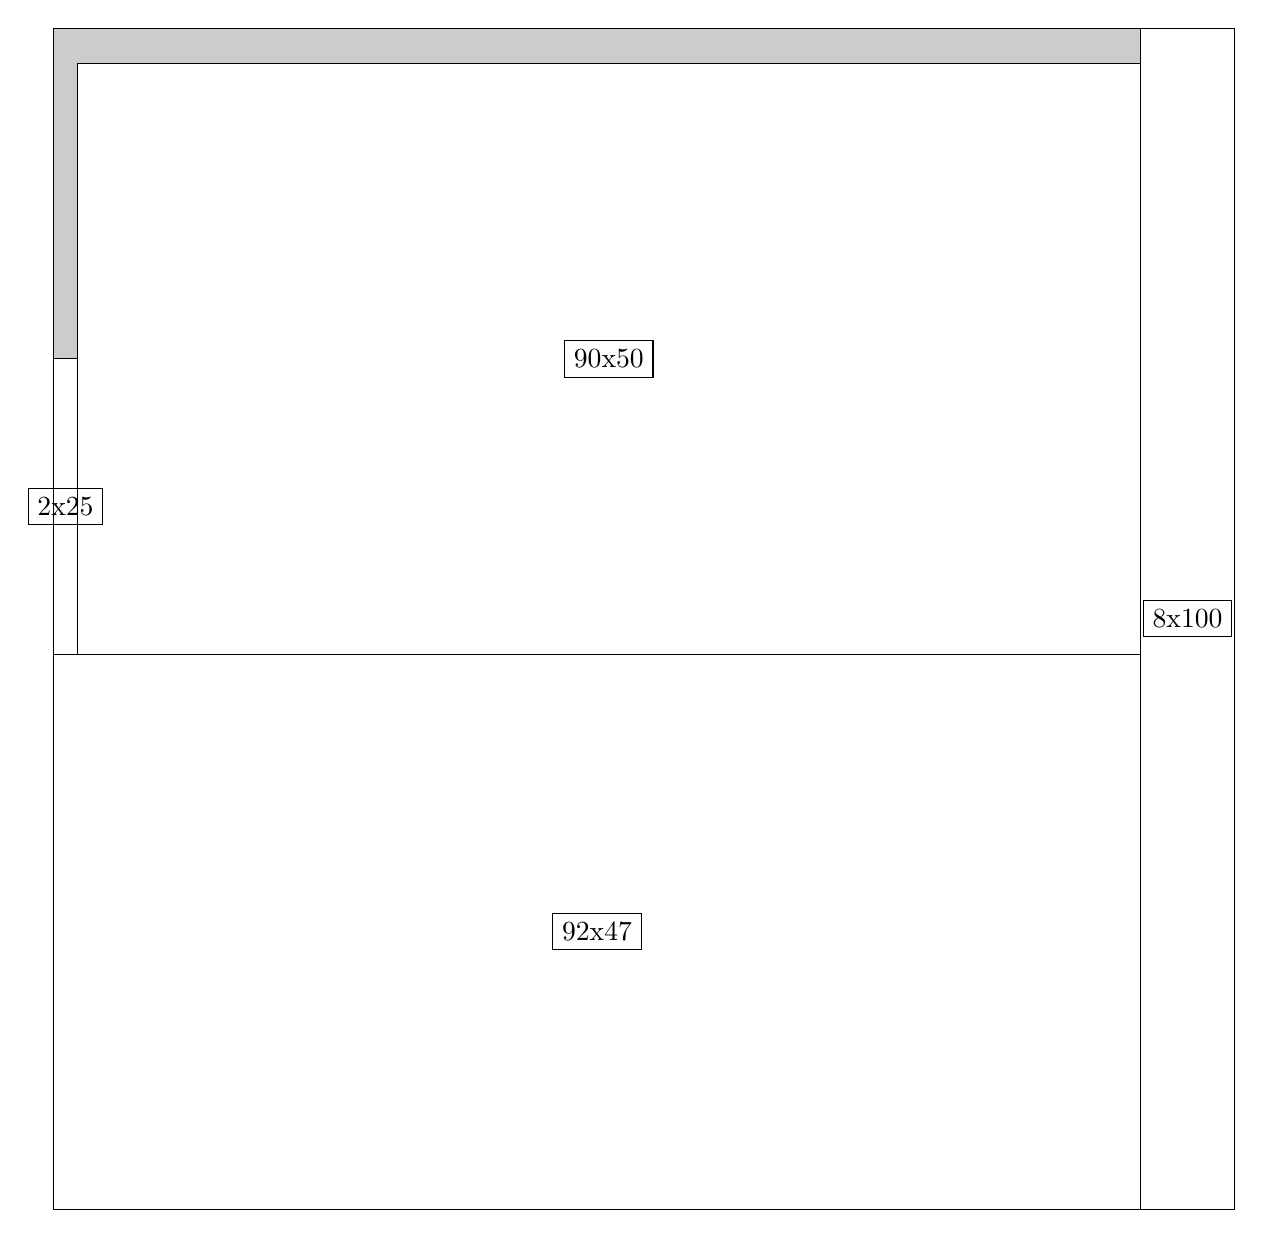
\begin{tikzpicture}[shorten >=1pt,scale=1.0,every node/.style={scale=1.0},->]
\tikzstyle{vertex}=[circle,fill=black!25,minimum size=14pt,inner sep=0pt]
\filldraw[fill=gray!40!white, draw=black] (0,0) rectangle (15.0,15.0);
\foreach \name/\x/\y/\w/\h in {8x100/13.799999999999999/0.0/1.2/15.0,92x47/0.0/0.0/13.799999999999999/7.05,90x50/0.3/7.05/13.5/7.5,2x25/0.0/7.05/0.3/3.75}
\filldraw[fill=white!40!white, draw=black] (\x,\y) rectangle node[draw] (\name) {\name} ++(\w,\h);
\end{tikzpicture}


w =8 , h =100 , x =92 , y =0 , v =800
\par
w =92 , h =47 , x =0 , y =0 , v =4324
\par
w =90 , h =50 , x =2 , y =47 , v =4500
\par
w =2 , h =25 , x =0 , y =47 , v =50
\par
\newpage


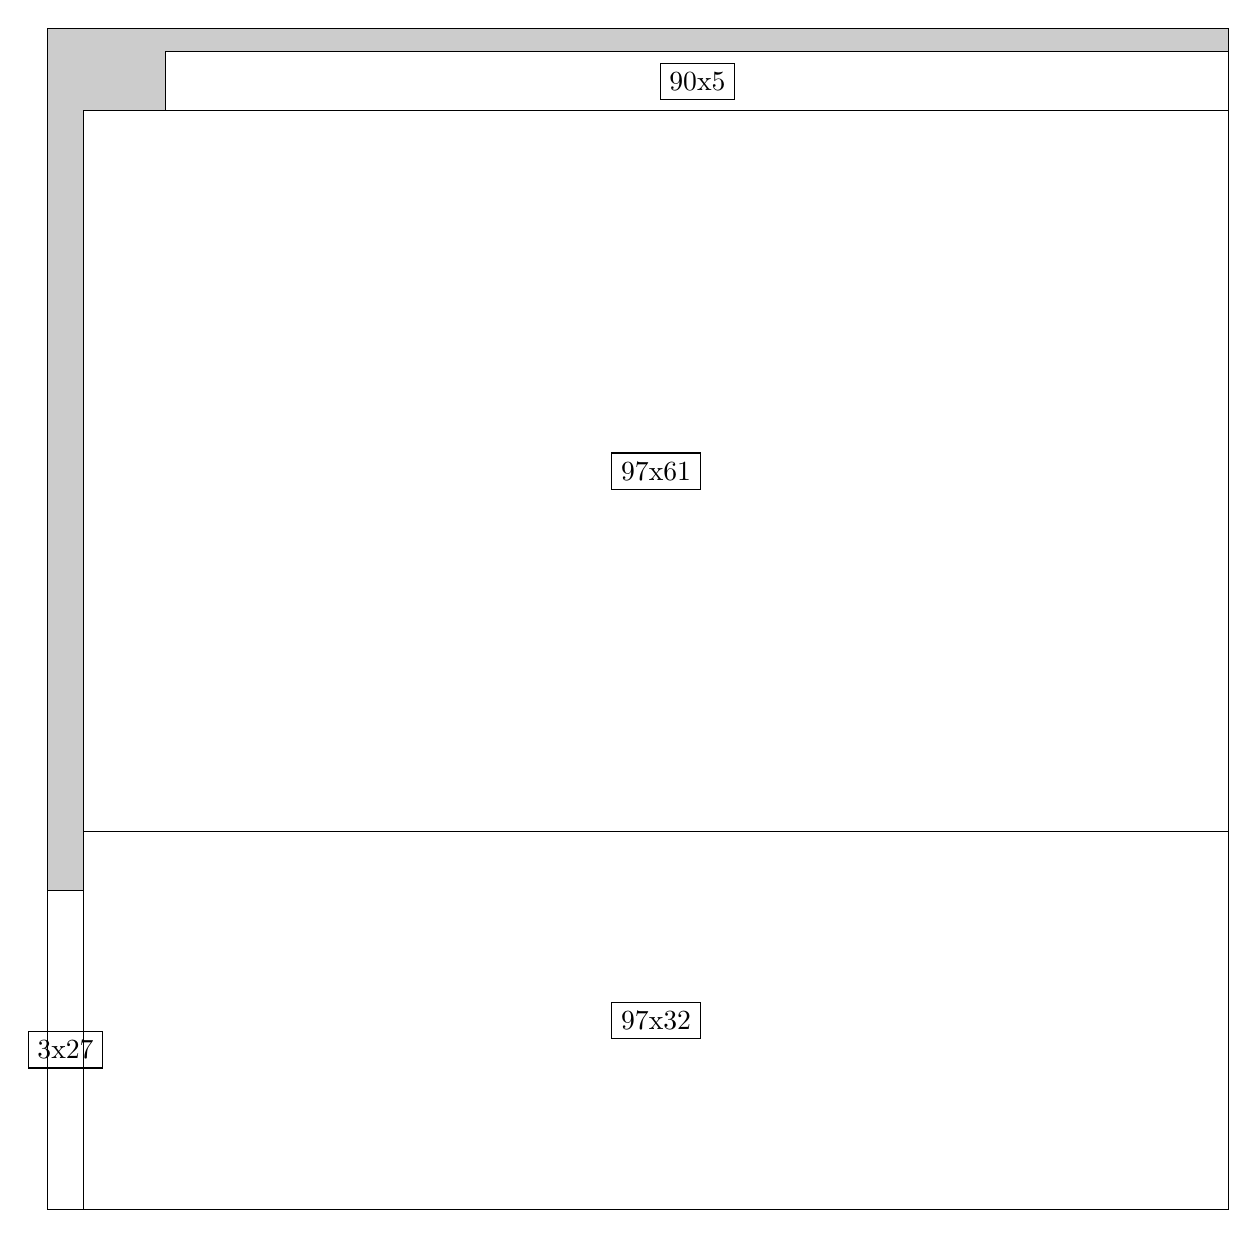
\begin{tikzpicture}[shorten >=1pt,scale=1.0,every node/.style={scale=1.0},->]
\tikzstyle{vertex}=[circle,fill=black!25,minimum size=14pt,inner sep=0pt]
\filldraw[fill=gray!40!white, draw=black] (0,0) rectangle (15.0,15.0);
\foreach \name/\x/\y/\w/\h in {97x32/0.44999999999999996/0.0/14.549999999999999/4.8,3x27/0.0/0.0/0.44999999999999996/4.05,97x61/0.44999999999999996/4.8/14.549999999999999/9.15,90x5/1.5/13.95/13.5/0.75}
\filldraw[fill=white!40!white, draw=black] (\x,\y) rectangle node[draw] (\name) {\name} ++(\w,\h);
\end{tikzpicture}


w =97 , h =32 , x =3 , y =0 , v =3104
\par
w =3 , h =27 , x =0 , y =0 , v =81
\par
w =97 , h =61 , x =3 , y =32 , v =5917
\par
w =90 , h =5 , x =10 , y =93 , v =450
\par
\newpage


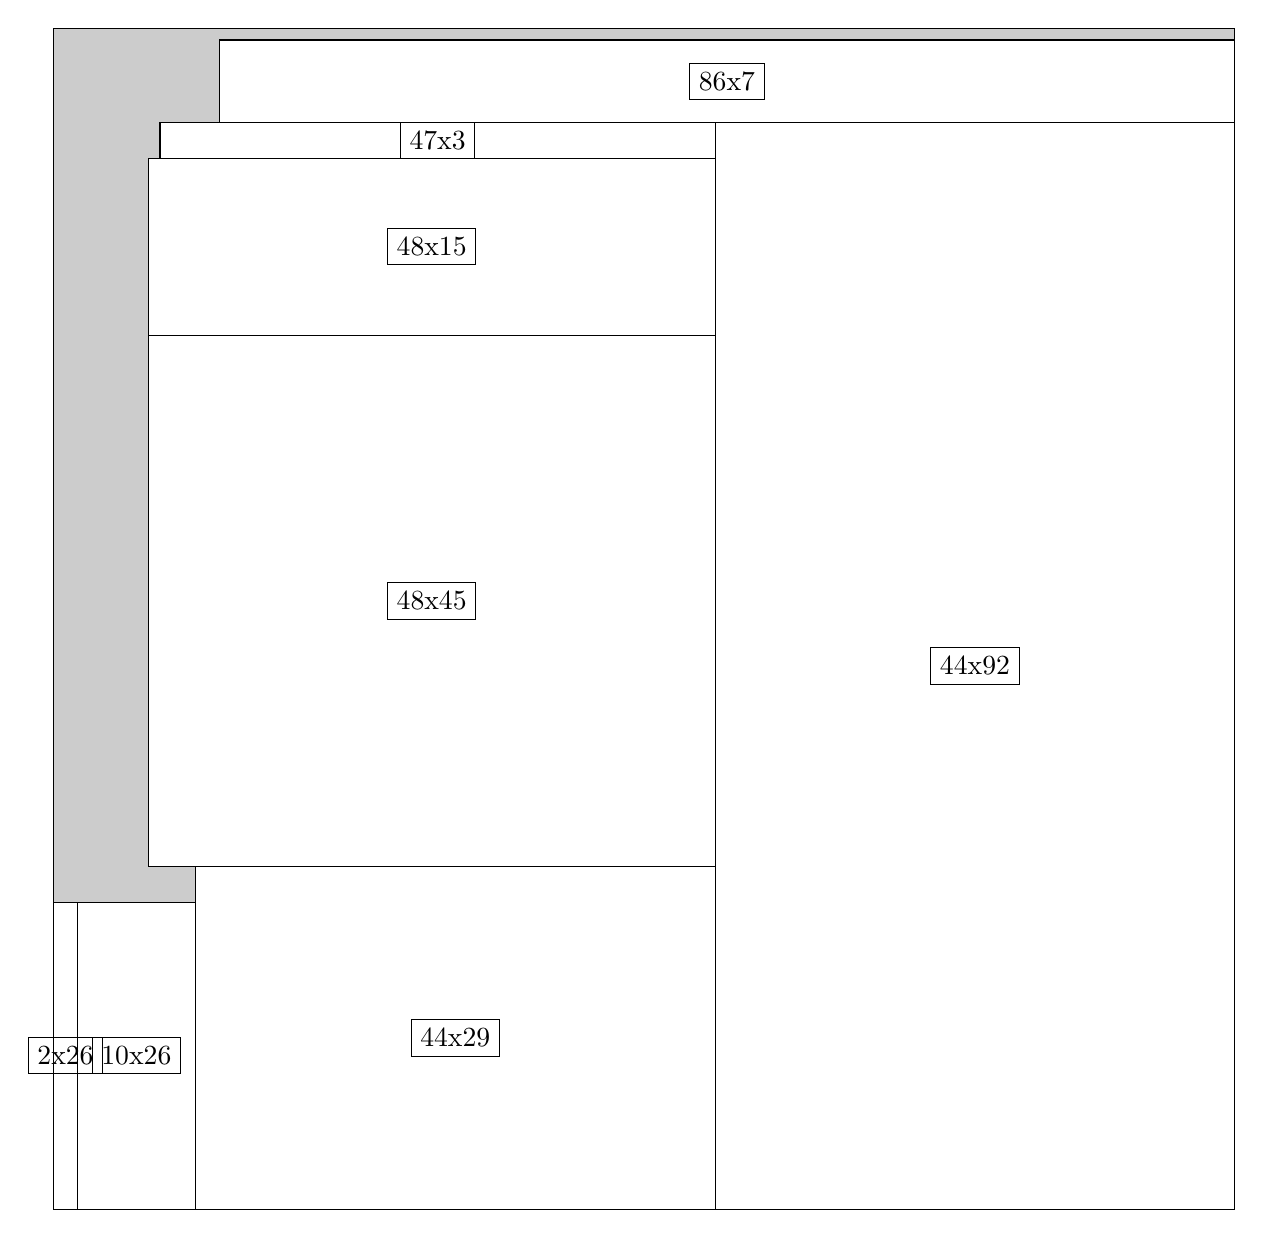
\begin{tikzpicture}[shorten >=1pt,scale=1.0,every node/.style={scale=1.0},->]
\tikzstyle{vertex}=[circle,fill=black!25,minimum size=14pt,inner sep=0pt]
\filldraw[fill=gray!40!white, draw=black] (0,0) rectangle (15.0,15.0);
\foreach \name/\x/\y/\w/\h in {44x92/8.4/0.0/6.6/13.799999999999999,44x29/1.7999999999999998/0.0/6.6/4.35,10x26/0.3/0.0/1.5/3.9,2x26/0.0/0.0/0.3/3.9,48x45/1.2/4.35/7.199999999999999/6.75,48x15/1.2/11.1/7.199999999999999/2.25,47x3/1.3499999999999999/13.35/7.05/0.44999999999999996,86x7/2.1/13.799999999999999/12.9/1.05}
\filldraw[fill=white!40!white, draw=black] (\x,\y) rectangle node[draw] (\name) {\name} ++(\w,\h);
\end{tikzpicture}


w =44 , h =92 , x =56 , y =0 , v =4048
\par
w =44 , h =29 , x =12 , y =0 , v =1276
\par
w =10 , h =26 , x =2 , y =0 , v =260
\par
w =2 , h =26 , x =0 , y =0 , v =52
\par
w =48 , h =45 , x =8 , y =29 , v =2160
\par
w =48 , h =15 , x =8 , y =74 , v =720
\par
w =47 , h =3 , x =9 , y =89 , v =141
\par
w =86 , h =7 , x =14 , y =92 , v =602
\par
\newpage


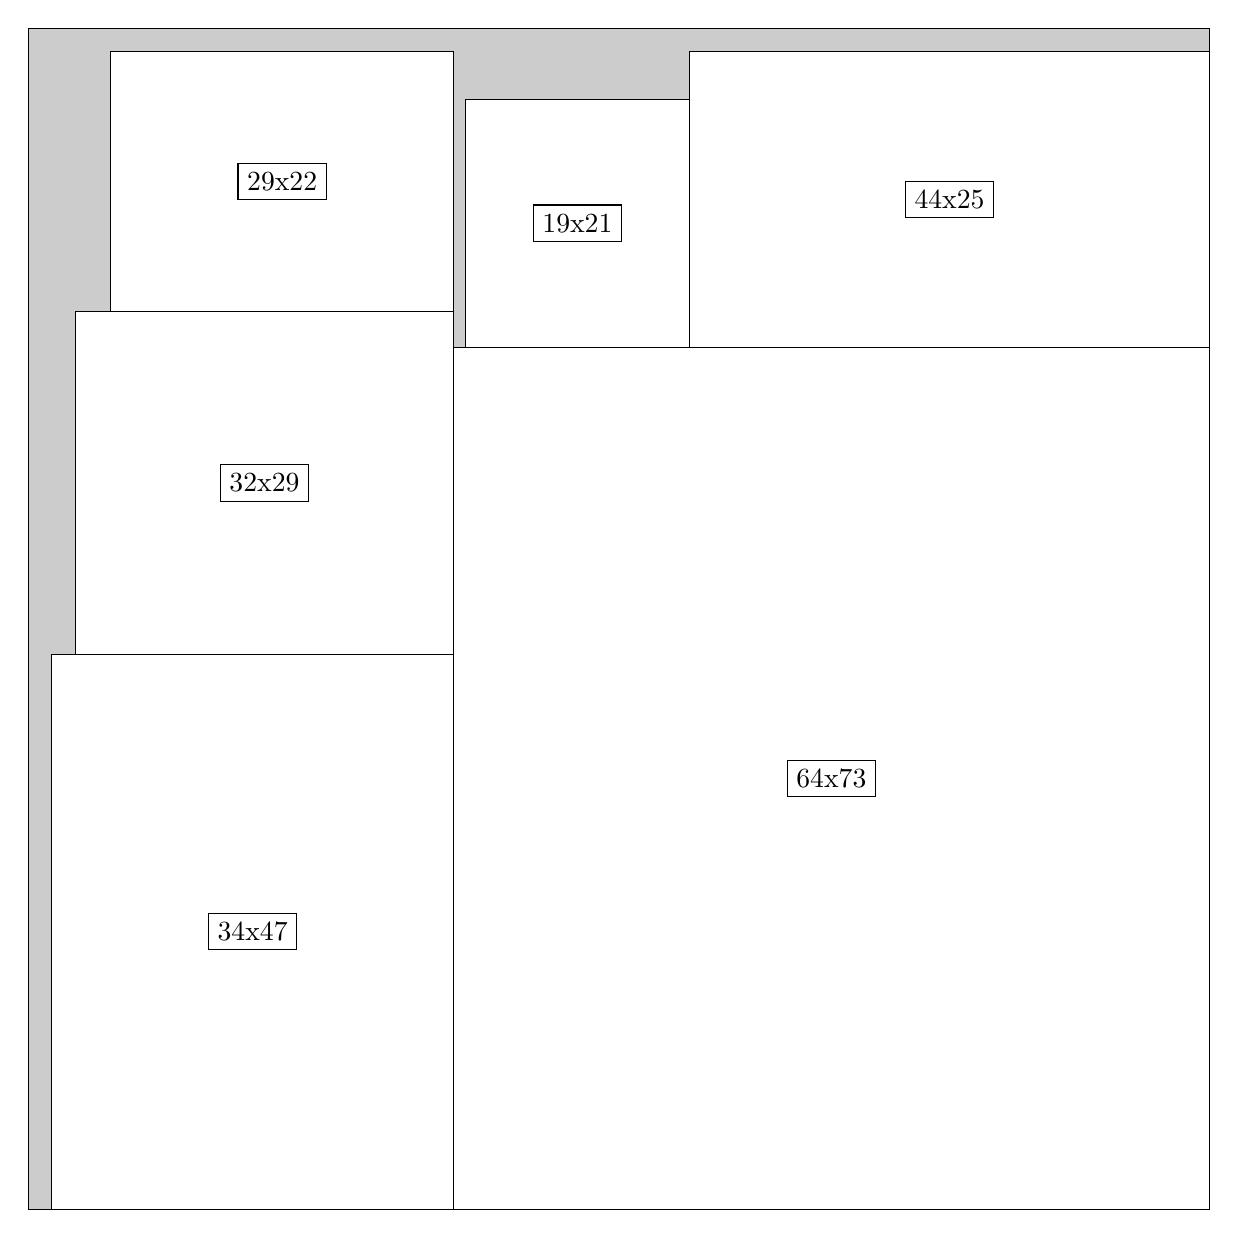
\begin{tikzpicture}[shorten >=1pt,scale=1.0,every node/.style={scale=1.0},->]
\tikzstyle{vertex}=[circle,fill=black!25,minimum size=14pt,inner sep=0pt]
\filldraw[fill=gray!40!white, draw=black] (0,0) rectangle (15.0,15.0);
\foreach \name/\x/\y/\w/\h in {64x73/5.3999999999999995/0.0/9.6/10.95,44x25/8.4/10.95/6.6/3.75,19x21/5.55/10.95/2.85/3.15,34x47/0.3/0.0/5.1/7.05,32x29/0.6/7.05/4.8/4.35,29x22/1.05/11.4/4.35/3.3}
\filldraw[fill=white!40!white, draw=black] (\x,\y) rectangle node[draw] (\name) {\name} ++(\w,\h);
\end{tikzpicture}


w =64 , h =73 , x =36 , y =0 , v =4672
\par
w =44 , h =25 , x =56 , y =73 , v =1100
\par
w =19 , h =21 , x =37 , y =73 , v =399
\par
w =34 , h =47 , x =2 , y =0 , v =1598
\par
w =32 , h =29 , x =4 , y =47 , v =928
\par
w =29 , h =22 , x =7 , y =76 , v =638
\par
\newpage


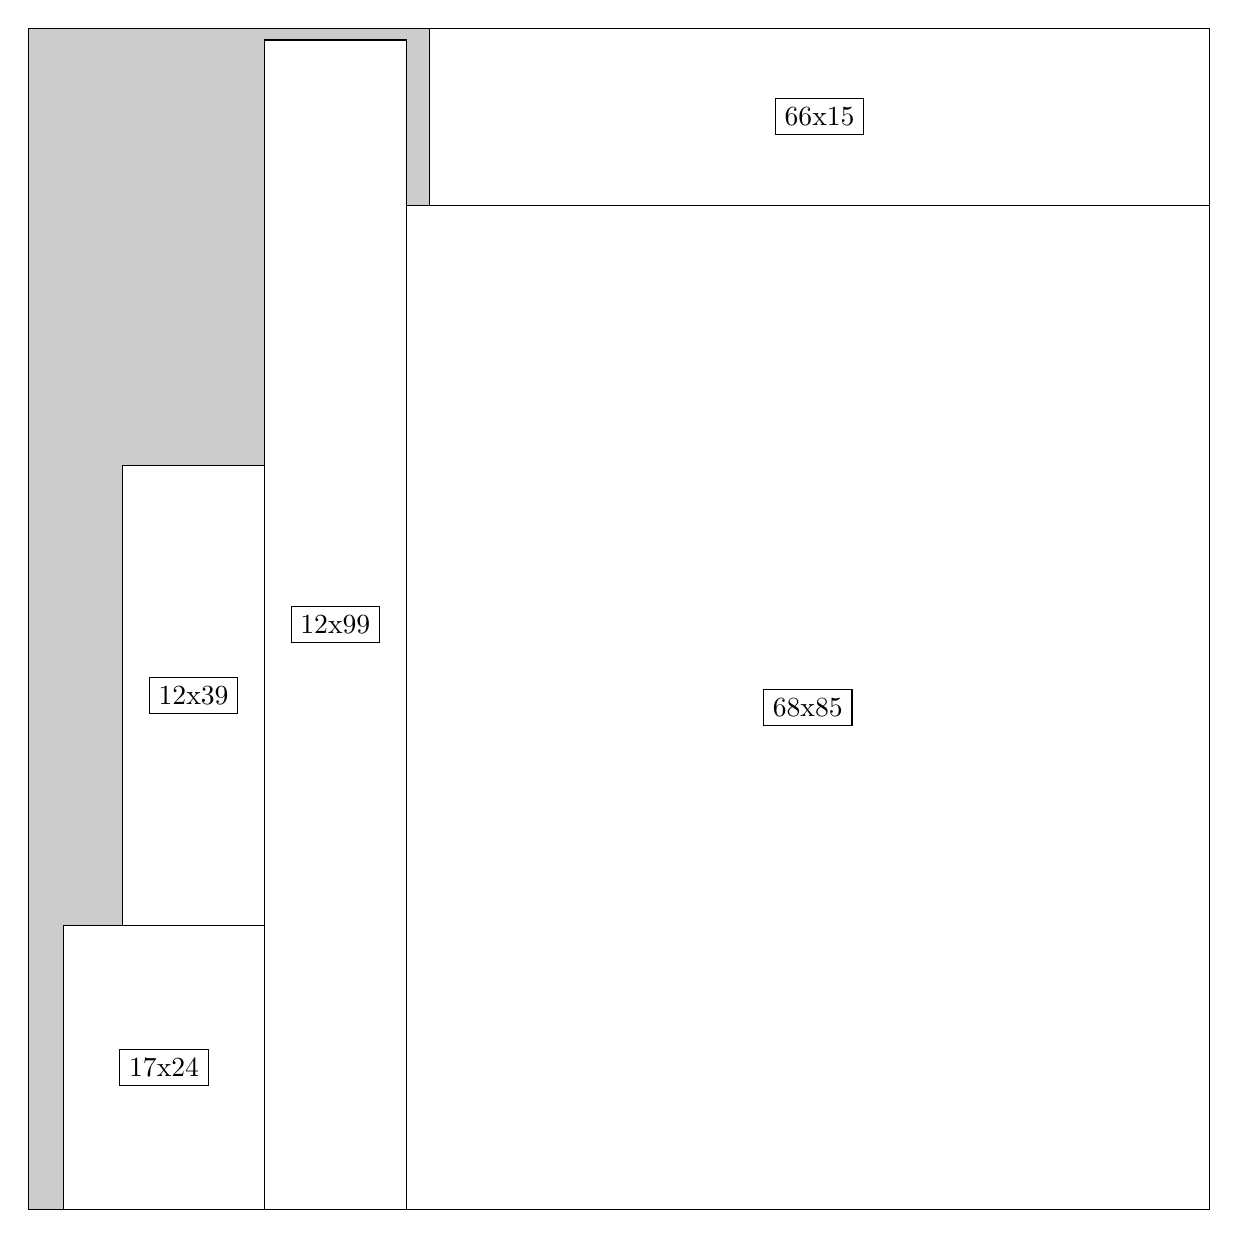
\begin{tikzpicture}[shorten >=1pt,scale=1.0,every node/.style={scale=1.0},->]
\tikzstyle{vertex}=[circle,fill=black!25,minimum size=14pt,inner sep=0pt]
\filldraw[fill=gray!40!white, draw=black] (0,0) rectangle (15.0,15.0);
\foreach \name/\x/\y/\w/\h in {68x85/4.8/0.0/10.2/12.75,66x15/5.1/12.75/9.9/2.25,12x99/3.0/0.0/1.7999999999999998/14.85,17x24/0.44999999999999996/0.0/2.55/3.5999999999999996,12x39/1.2/3.5999999999999996/1.7999999999999998/5.85}
\filldraw[fill=white!40!white, draw=black] (\x,\y) rectangle node[draw] (\name) {\name} ++(\w,\h);
\end{tikzpicture}


w =68 , h =85 , x =32 , y =0 , v =5780
\par
w =66 , h =15 , x =34 , y =85 , v =990
\par
w =12 , h =99 , x =20 , y =0 , v =1188
\par
w =17 , h =24 , x =3 , y =0 , v =408
\par
w =12 , h =39 , x =8 , y =24 , v =468
\par
\newpage


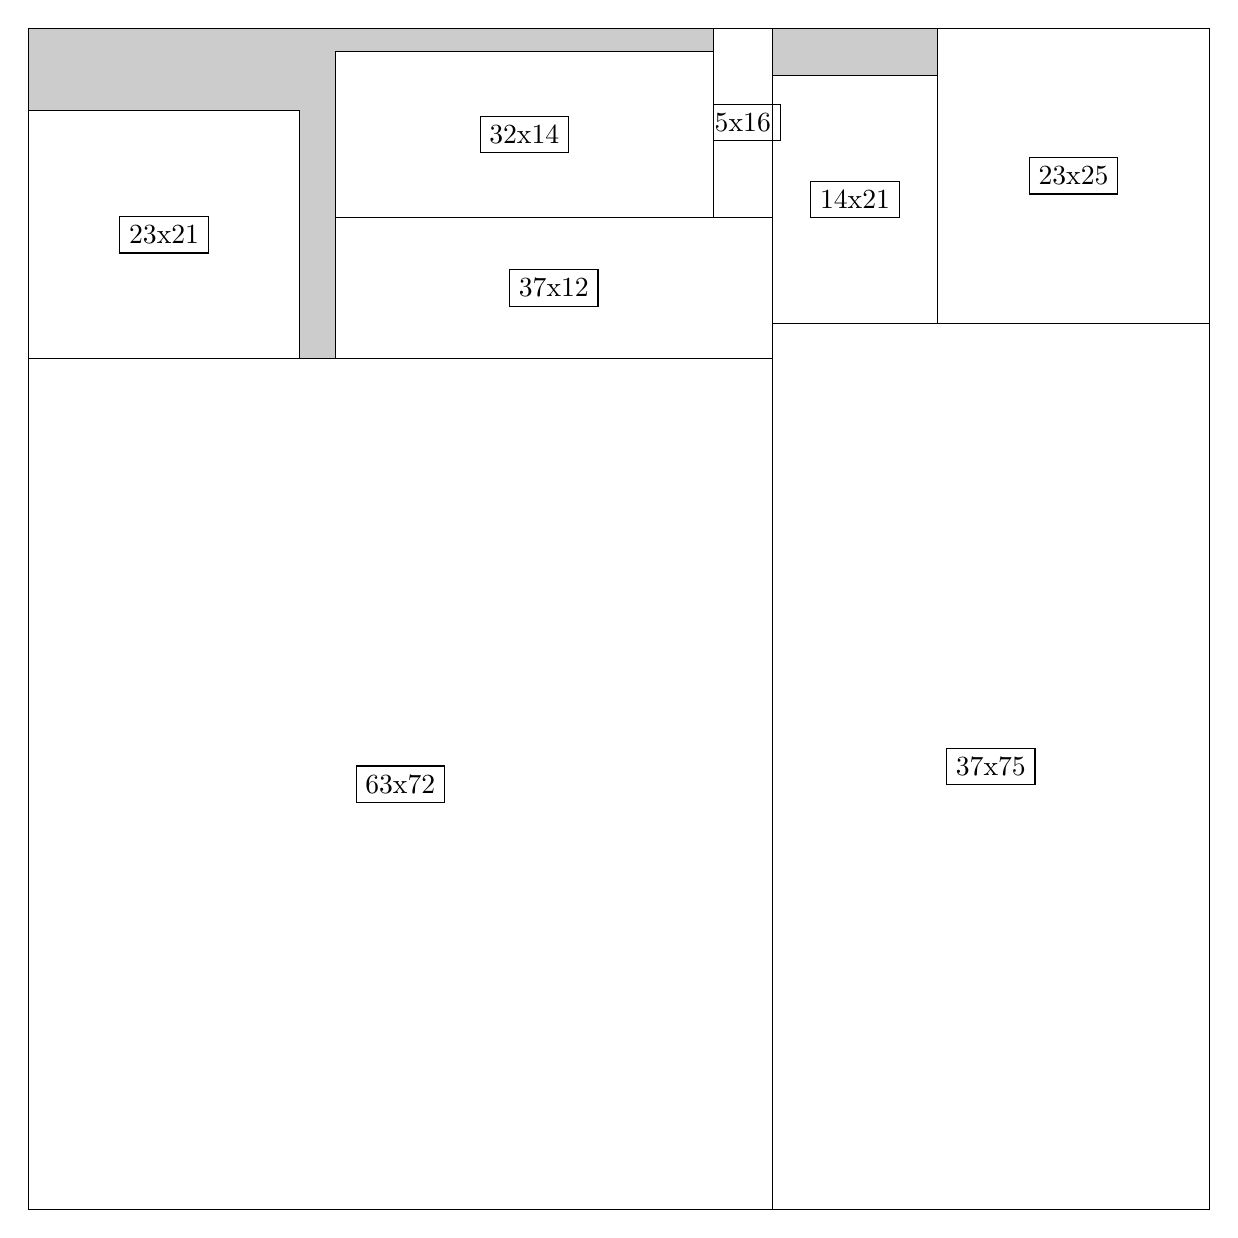
\begin{tikzpicture}[shorten >=1pt,scale=1.0,every node/.style={scale=1.0},->]
\tikzstyle{vertex}=[circle,fill=black!25,minimum size=14pt,inner sep=0pt]
\filldraw[fill=gray!40!white, draw=black] (0,0) rectangle (15.0,15.0);
\foreach \name/\x/\y/\w/\h in {37x75/9.45/0.0/5.55/11.25,23x25/11.549999999999999/11.25/3.4499999999999997/3.75,14x21/9.45/11.25/2.1/3.15,63x72/0.0/0.0/9.45/10.799999999999999,37x12/3.9/10.799999999999999/5.55/1.7999999999999998,5x16/8.7/12.6/0.75/2.4,32x14/3.9/12.6/4.8/2.1,23x21/0.0/10.799999999999999/3.4499999999999997/3.15}
\filldraw[fill=white!40!white, draw=black] (\x,\y) rectangle node[draw] (\name) {\name} ++(\w,\h);
\end{tikzpicture}


w =37 , h =75 , x =63 , y =0 , v =2775
\par
w =23 , h =25 , x =77 , y =75 , v =575
\par
w =14 , h =21 , x =63 , y =75 , v =294
\par
w =63 , h =72 , x =0 , y =0 , v =4536
\par
w =37 , h =12 , x =26 , y =72 , v =444
\par
w =5 , h =16 , x =58 , y =84 , v =80
\par
w =32 , h =14 , x =26 , y =84 , v =448
\par
w =23 , h =21 , x =0 , y =72 , v =483
\par
\newpage


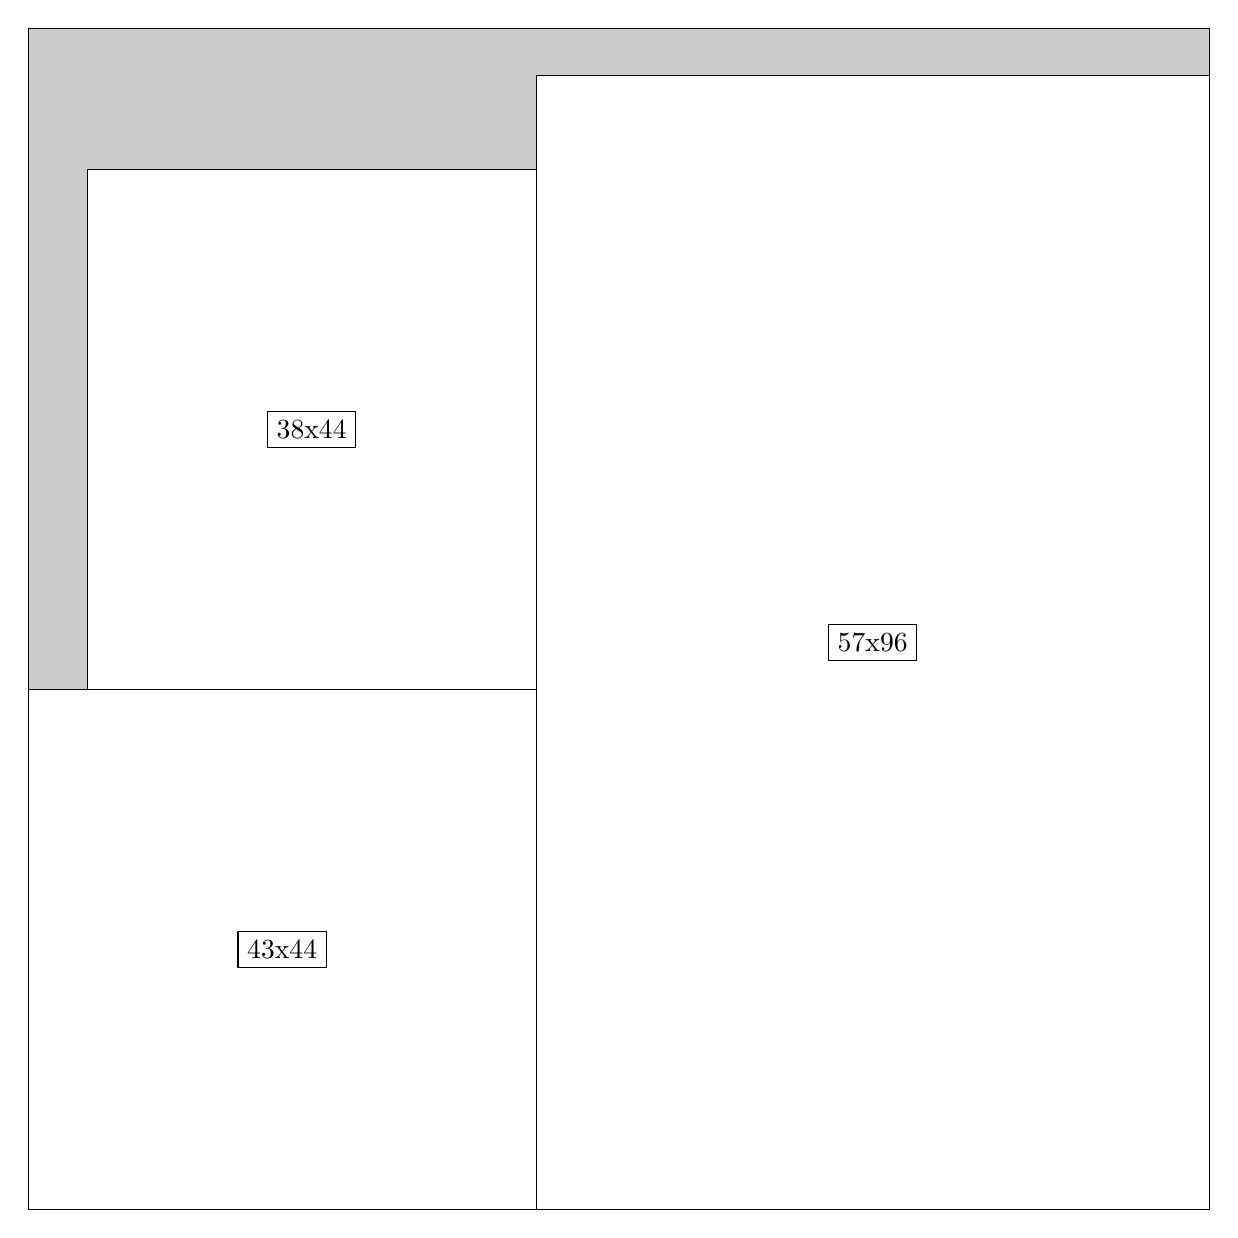
\begin{tikzpicture}[shorten >=1pt,scale=1.0,every node/.style={scale=1.0},->]
\tikzstyle{vertex}=[circle,fill=black!25,minimum size=14pt,inner sep=0pt]
\filldraw[fill=gray!40!white, draw=black] (0,0) rectangle (15.0,15.0);
\foreach \name/\x/\y/\w/\h in {57x96/6.45/0.0/8.549999999999999/14.399999999999999,43x44/0.0/0.0/6.45/6.6,38x44/0.75/6.6/5.7/6.6}
\filldraw[fill=white!40!white, draw=black] (\x,\y) rectangle node[draw] (\name) {\name} ++(\w,\h);
\end{tikzpicture}


w =57 , h =96 , x =43 , y =0 , v =5472
\par
w =43 , h =44 , x =0 , y =0 , v =1892
\par
w =38 , h =44 , x =5 , y =44 , v =1672
\par
\newpage


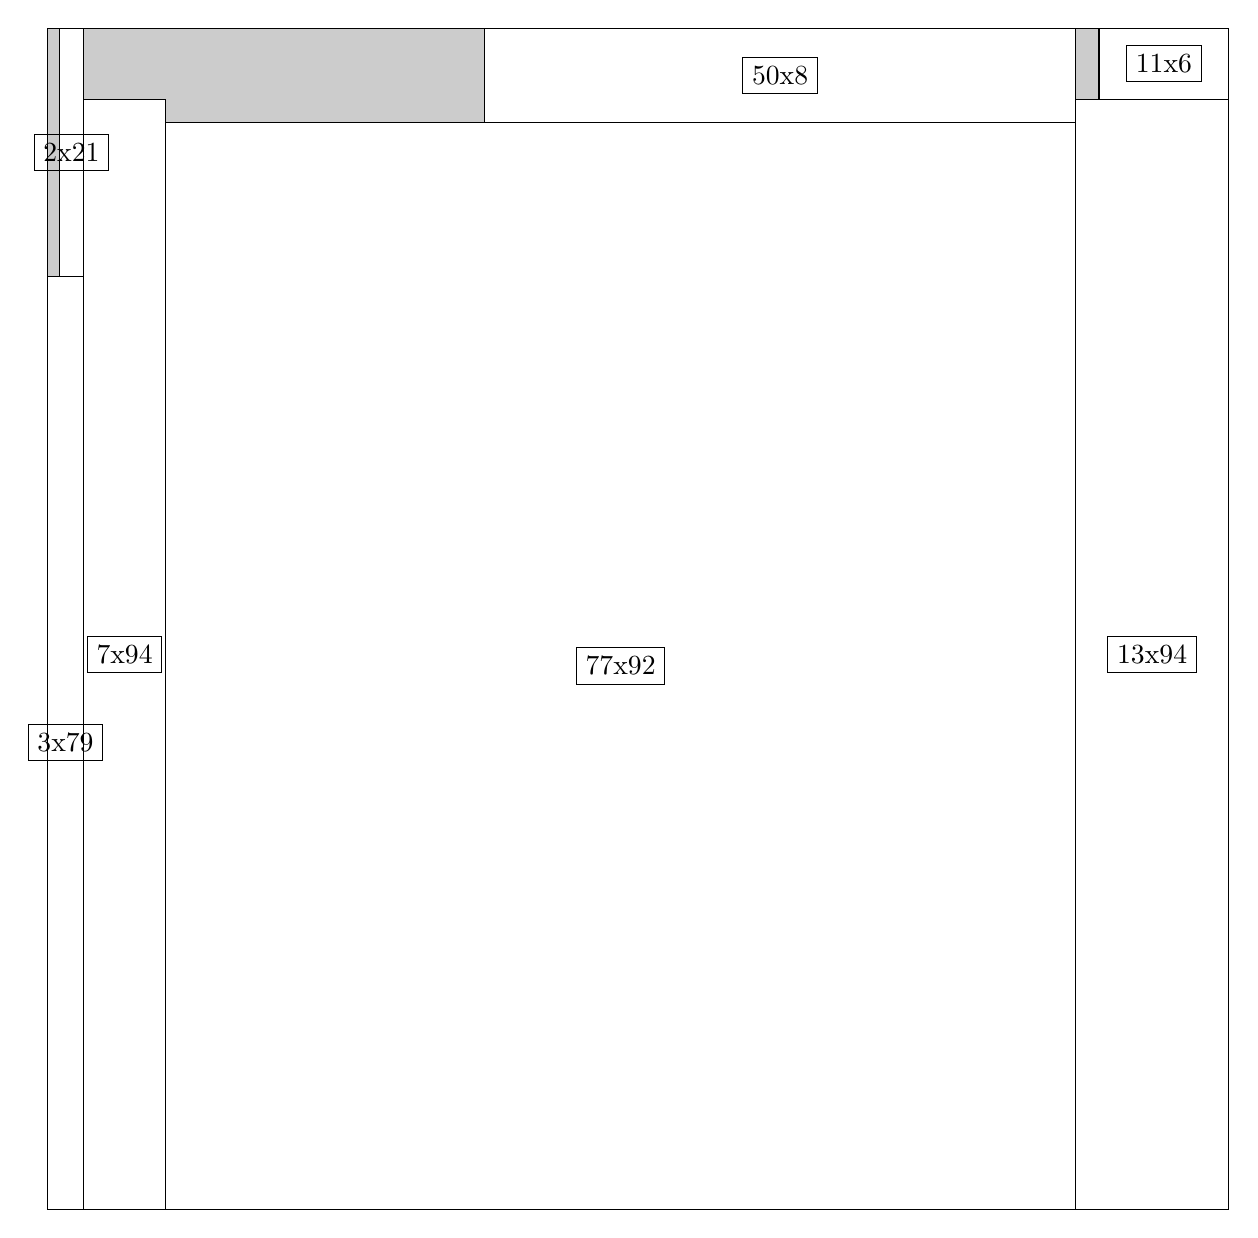
\begin{tikzpicture}[shorten >=1pt,scale=1.0,every node/.style={scale=1.0},->]
\tikzstyle{vertex}=[circle,fill=black!25,minimum size=14pt,inner sep=0pt]
\filldraw[fill=gray!40!white, draw=black] (0,0) rectangle (15.0,15.0);
\foreach \name/\x/\y/\w/\h in {13x94/13.049999999999999/0.0/1.95/14.1,11x6/13.35/14.1/1.65/0.8999999999999999,77x92/1.5/0.0/11.549999999999999/13.799999999999999,50x8/5.55/13.799999999999999/7.5/1.2,7x94/0.44999999999999996/0.0/1.05/14.1,3x79/0.0/0.0/0.44999999999999996/11.85,2x21/0.15/11.85/0.3/3.15}
\filldraw[fill=white!40!white, draw=black] (\x,\y) rectangle node[draw] (\name) {\name} ++(\w,\h);
\end{tikzpicture}


w =13 , h =94 , x =87 , y =0 , v =1222
\par
w =11 , h =6 , x =89 , y =94 , v =66
\par
w =77 , h =92 , x =10 , y =0 , v =7084
\par
w =50 , h =8 , x =37 , y =92 , v =400
\par
w =7 , h =94 , x =3 , y =0 , v =658
\par
w =3 , h =79 , x =0 , y =0 , v =237
\par
w =2 , h =21 , x =1 , y =79 , v =42
\par
\newpage


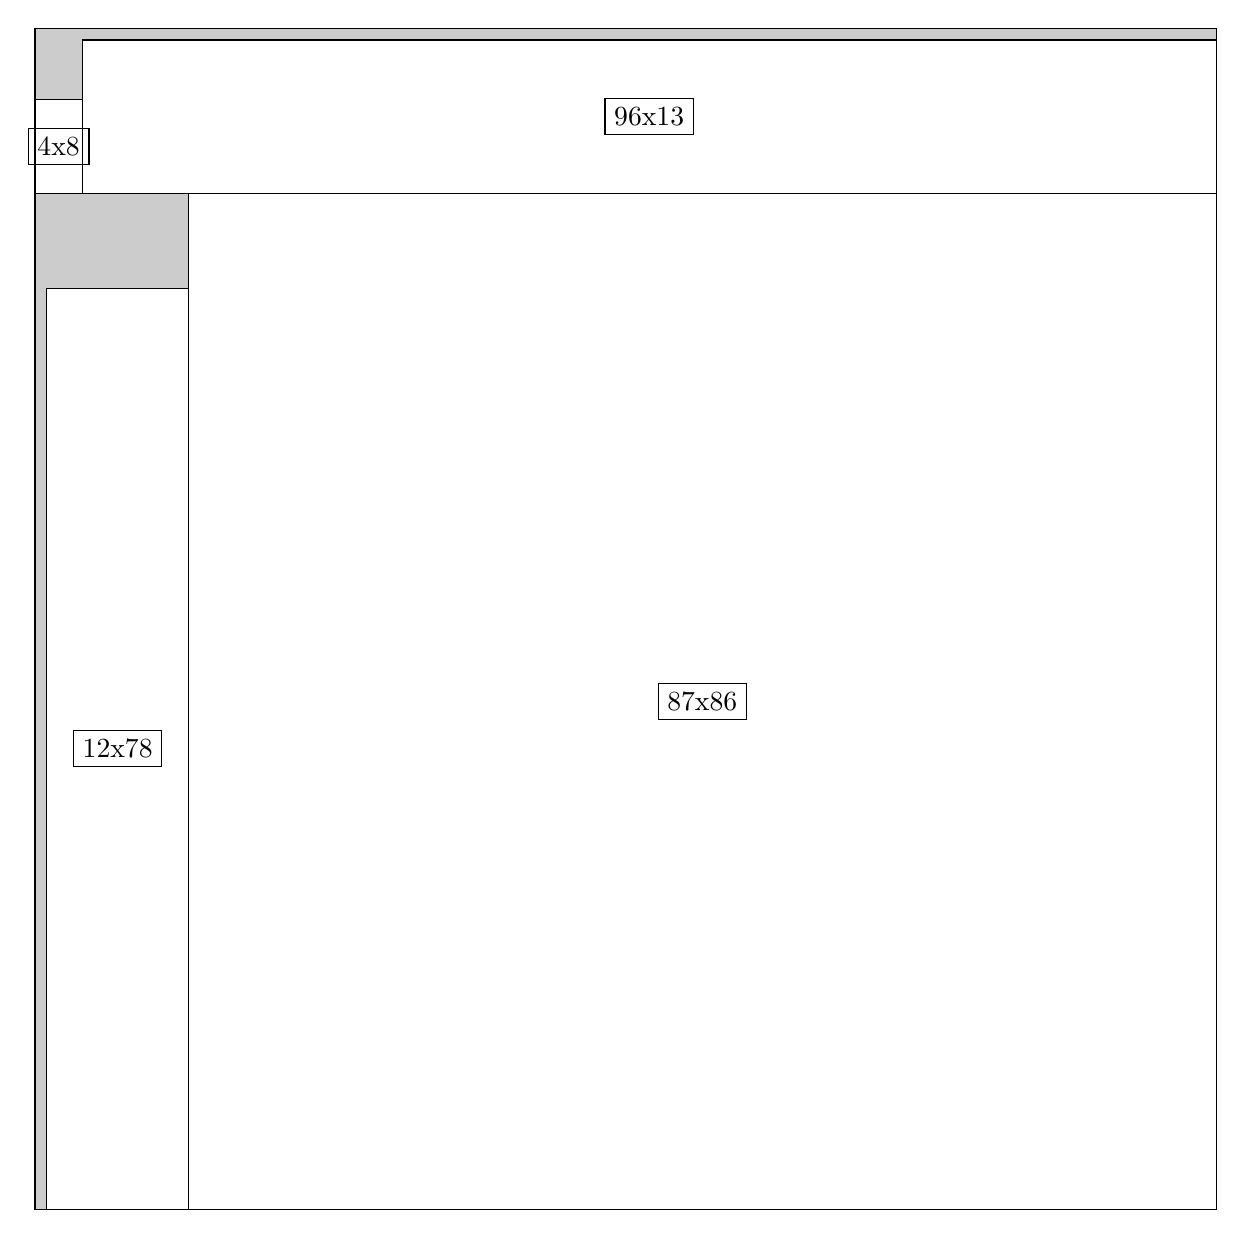
\begin{tikzpicture}[shorten >=1pt,scale=1.0,every node/.style={scale=1.0},->]
\tikzstyle{vertex}=[circle,fill=black!25,minimum size=14pt,inner sep=0pt]
\filldraw[fill=gray!40!white, draw=black] (0,0) rectangle (15.0,15.0);
\foreach \name/\x/\y/\w/\h in {87x86/1.95/0.0/13.049999999999999/12.9,12x78/0.15/0.0/1.7999999999999998/11.7,96x13/0.6/12.9/14.399999999999999/1.95,4x8/0.0/12.9/0.6/1.2}
\filldraw[fill=white!40!white, draw=black] (\x,\y) rectangle node[draw] (\name) {\name} ++(\w,\h);
\end{tikzpicture}


w =87 , h =86 , x =13 , y =0 , v =7482
\par
w =12 , h =78 , x =1 , y =0 , v =936
\par
w =96 , h =13 , x =4 , y =86 , v =1248
\par
w =4 , h =8 , x =0 , y =86 , v =32
\par
\newpage


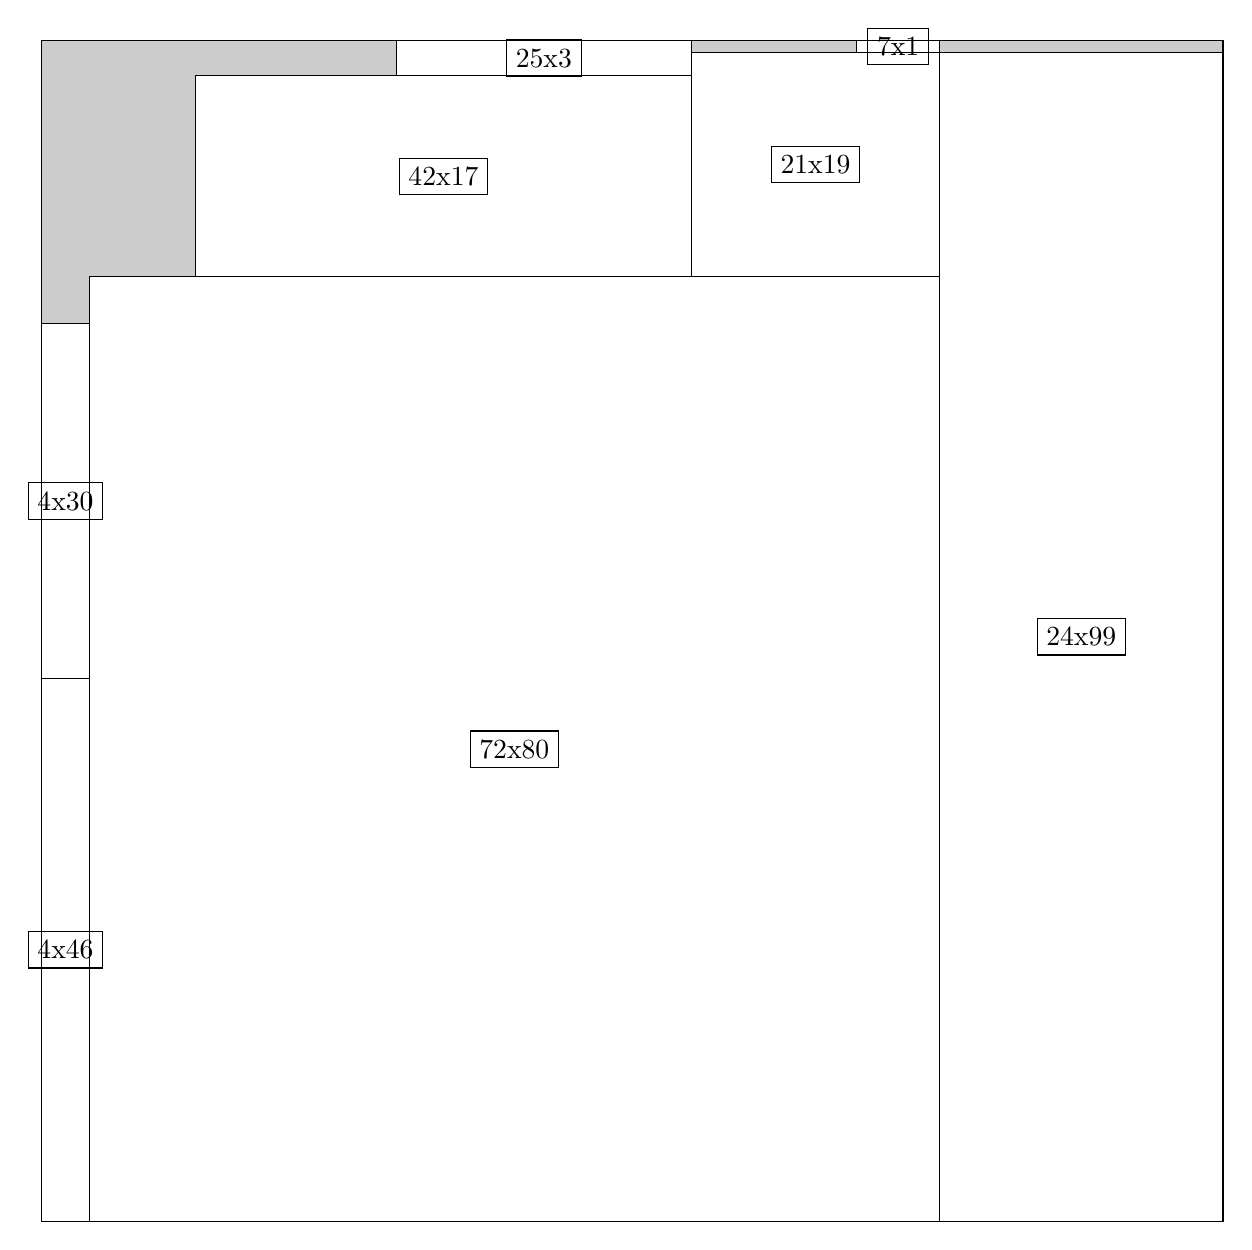
\begin{tikzpicture}[shorten >=1pt,scale=1.0,every node/.style={scale=1.0},->]
\tikzstyle{vertex}=[circle,fill=black!25,minimum size=14pt,inner sep=0pt]
\filldraw[fill=gray!40!white, draw=black] (0,0) rectangle (15.0,15.0);
\foreach \name/\x/\y/\w/\h in {24x99/11.4/0.0/3.5999999999999996/14.85,72x80/0.6/0.0/10.799999999999999/12.0,21x19/8.25/12.0/3.15/2.85,7x1/10.35/14.85/1.05/0.15,42x17/1.95/12.0/6.3/2.55,25x3/4.5/14.549999999999999/3.75/0.44999999999999996,4x46/0.0/0.0/0.6/6.8999999999999995,4x30/0.0/6.8999999999999995/0.6/4.5}
\filldraw[fill=white!40!white, draw=black] (\x,\y) rectangle node[draw] (\name) {\name} ++(\w,\h);
\end{tikzpicture}


w =24 , h =99 , x =76 , y =0 , v =2376
\par
w =72 , h =80 , x =4 , y =0 , v =5760
\par
w =21 , h =19 , x =55 , y =80 , v =399
\par
w =7 , h =1 , x =69 , y =99 , v =7
\par
w =42 , h =17 , x =13 , y =80 , v =714
\par
w =25 , h =3 , x =30 , y =97 , v =75
\par
w =4 , h =46 , x =0 , y =0 , v =184
\par
w =4 , h =30 , x =0 , y =46 , v =120
\par
\newpage


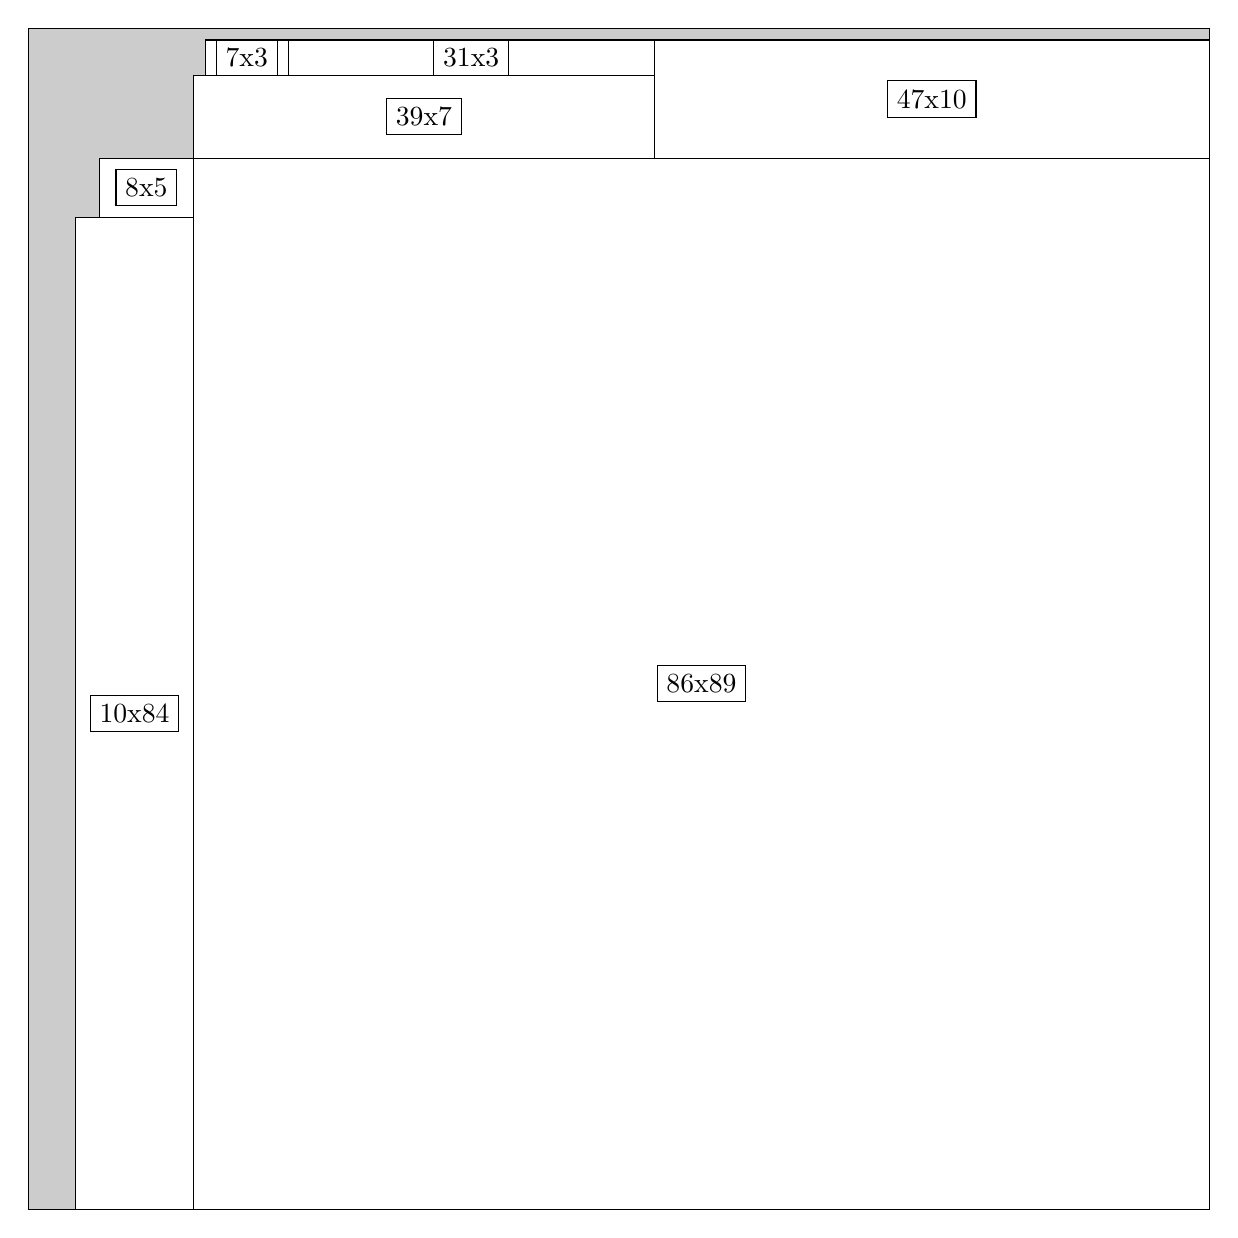
\begin{tikzpicture}[shorten >=1pt,scale=1.0,every node/.style={scale=1.0},->]
\tikzstyle{vertex}=[circle,fill=black!25,minimum size=14pt,inner sep=0pt]
\filldraw[fill=gray!40!white, draw=black] (0,0) rectangle (15.0,15.0);
\foreach \name/\x/\y/\w/\h in {86x89/2.1/0.0/12.9/13.35,10x84/0.6/0.0/1.5/12.6,8x5/0.8999999999999999/12.6/1.2/0.75,47x10/7.949999999999999/13.35/7.05/1.5,39x7/2.1/13.35/5.85/1.05,31x3/3.3/14.399999999999999/4.6499999999999995/0.44999999999999996,7x3/2.25/14.399999999999999/1.05/0.44999999999999996}
\filldraw[fill=white!40!white, draw=black] (\x,\y) rectangle node[draw] (\name) {\name} ++(\w,\h);
\end{tikzpicture}


w =86 , h =89 , x =14 , y =0 , v =7654
\par
w =10 , h =84 , x =4 , y =0 , v =840
\par
w =8 , h =5 , x =6 , y =84 , v =40
\par
w =47 , h =10 , x =53 , y =89 , v =470
\par
w =39 , h =7 , x =14 , y =89 , v =273
\par
w =31 , h =3 , x =22 , y =96 , v =93
\par
w =7 , h =3 , x =15 , y =96 , v =21
\par
\newpage


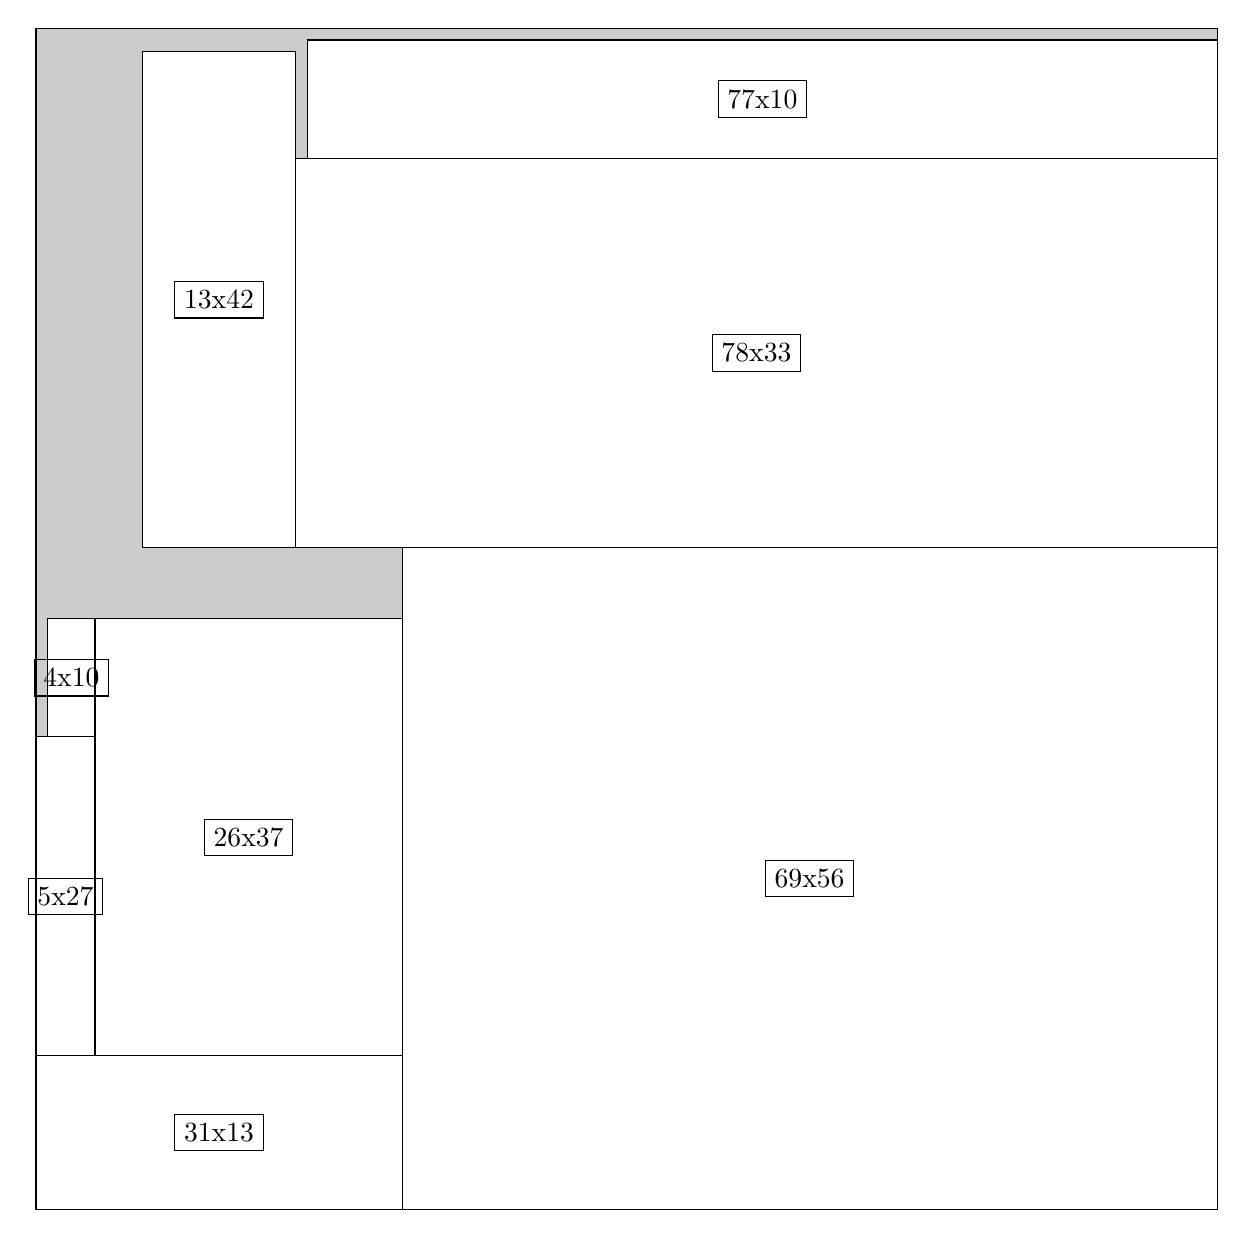
\begin{tikzpicture}[shorten >=1pt,scale=1.0,every node/.style={scale=1.0},->]
\tikzstyle{vertex}=[circle,fill=black!25,minimum size=14pt,inner sep=0pt]
\filldraw[fill=gray!40!white, draw=black] (0,0) rectangle (15.0,15.0);
\foreach \name/\x/\y/\w/\h in {69x56/4.6499999999999995/0.0/10.35/8.4,31x13/0.0/0.0/4.6499999999999995/1.95,26x37/0.75/1.95/3.9/5.55,5x27/0.0/1.95/0.75/4.05,4x10/0.15/6.0/0.6/1.5,78x33/3.3/8.4/11.7/4.95,77x10/3.4499999999999997/13.35/11.549999999999999/1.5,13x42/1.3499999999999999/8.4/1.95/6.3}
\filldraw[fill=white!40!white, draw=black] (\x,\y) rectangle node[draw] (\name) {\name} ++(\w,\h);
\end{tikzpicture}


w =69 , h =56 , x =31 , y =0 , v =3864
\par
w =31 , h =13 , x =0 , y =0 , v =403
\par
w =26 , h =37 , x =5 , y =13 , v =962
\par
w =5 , h =27 , x =0 , y =13 , v =135
\par
w =4 , h =10 , x =1 , y =40 , v =40
\par
w =78 , h =33 , x =22 , y =56 , v =2574
\par
w =77 , h =10 , x =23 , y =89 , v =770
\par
w =13 , h =42 , x =9 , y =56 , v =546
\par
\newpage


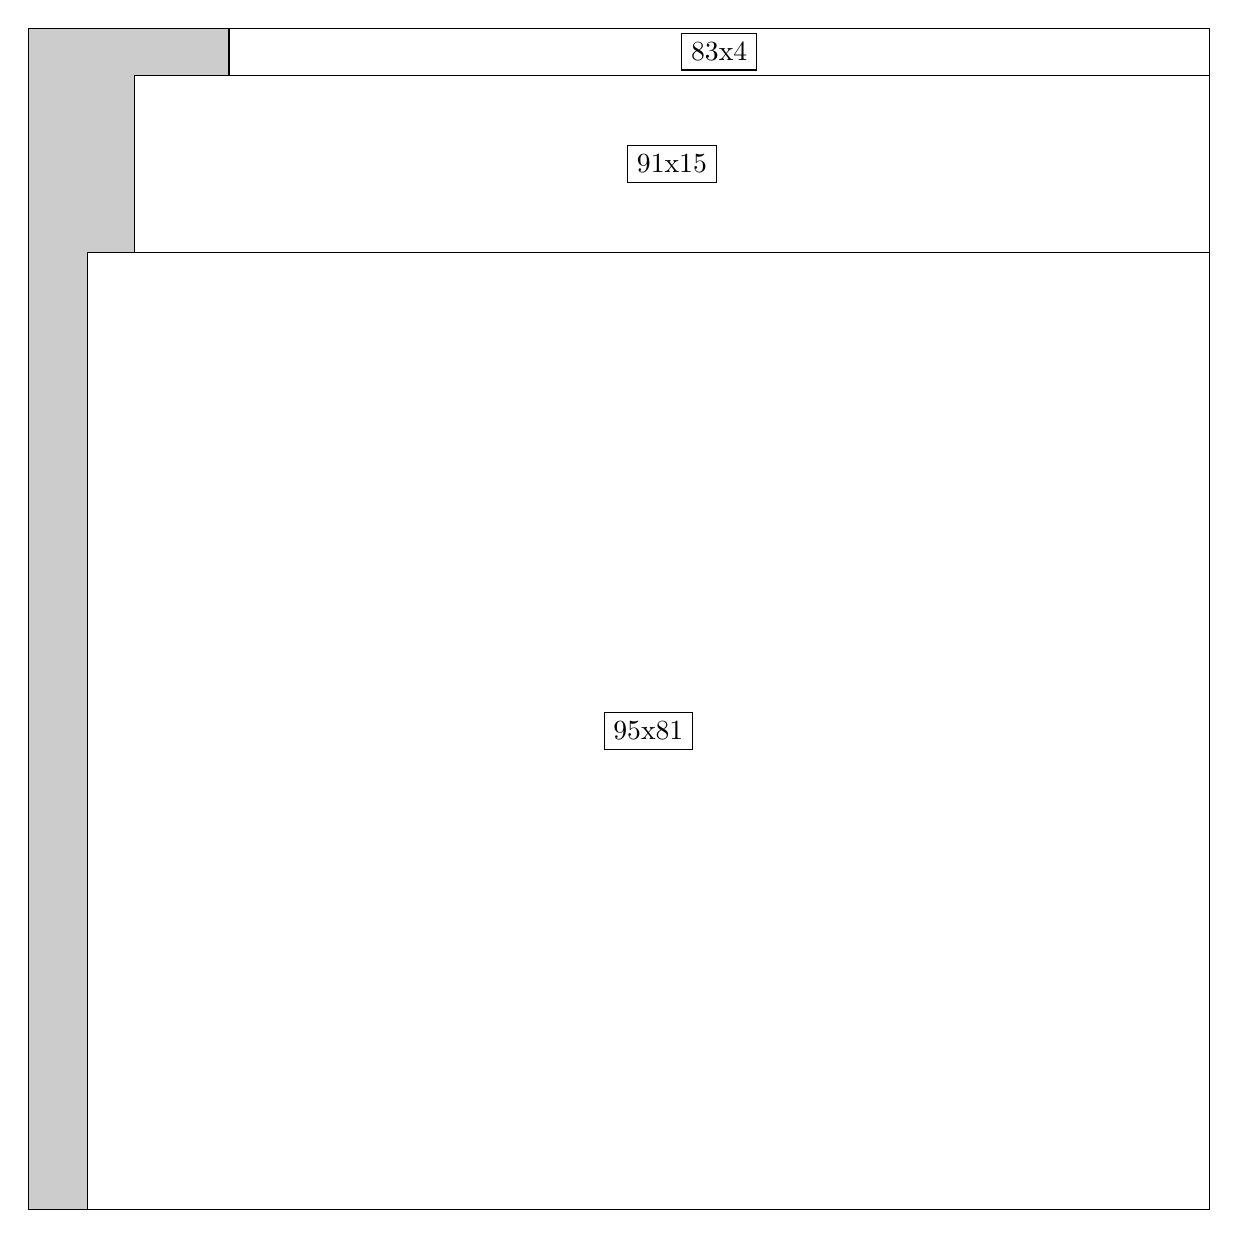
\begin{tikzpicture}[shorten >=1pt,scale=1.0,every node/.style={scale=1.0},->]
\tikzstyle{vertex}=[circle,fill=black!25,minimum size=14pt,inner sep=0pt]
\filldraw[fill=gray!40!white, draw=black] (0,0) rectangle (15.0,15.0);
\foreach \name/\x/\y/\w/\h in {95x81/0.75/0.0/14.25/12.15,91x15/1.3499999999999999/12.15/13.65/2.25,83x4/2.55/14.399999999999999/12.45/0.6}
\filldraw[fill=white!40!white, draw=black] (\x,\y) rectangle node[draw] (\name) {\name} ++(\w,\h);
\end{tikzpicture}


w =95 , h =81 , x =5 , y =0 , v =7695
\par
w =91 , h =15 , x =9 , y =81 , v =1365
\par
w =83 , h =4 , x =17 , y =96 , v =332
\par
\newpage


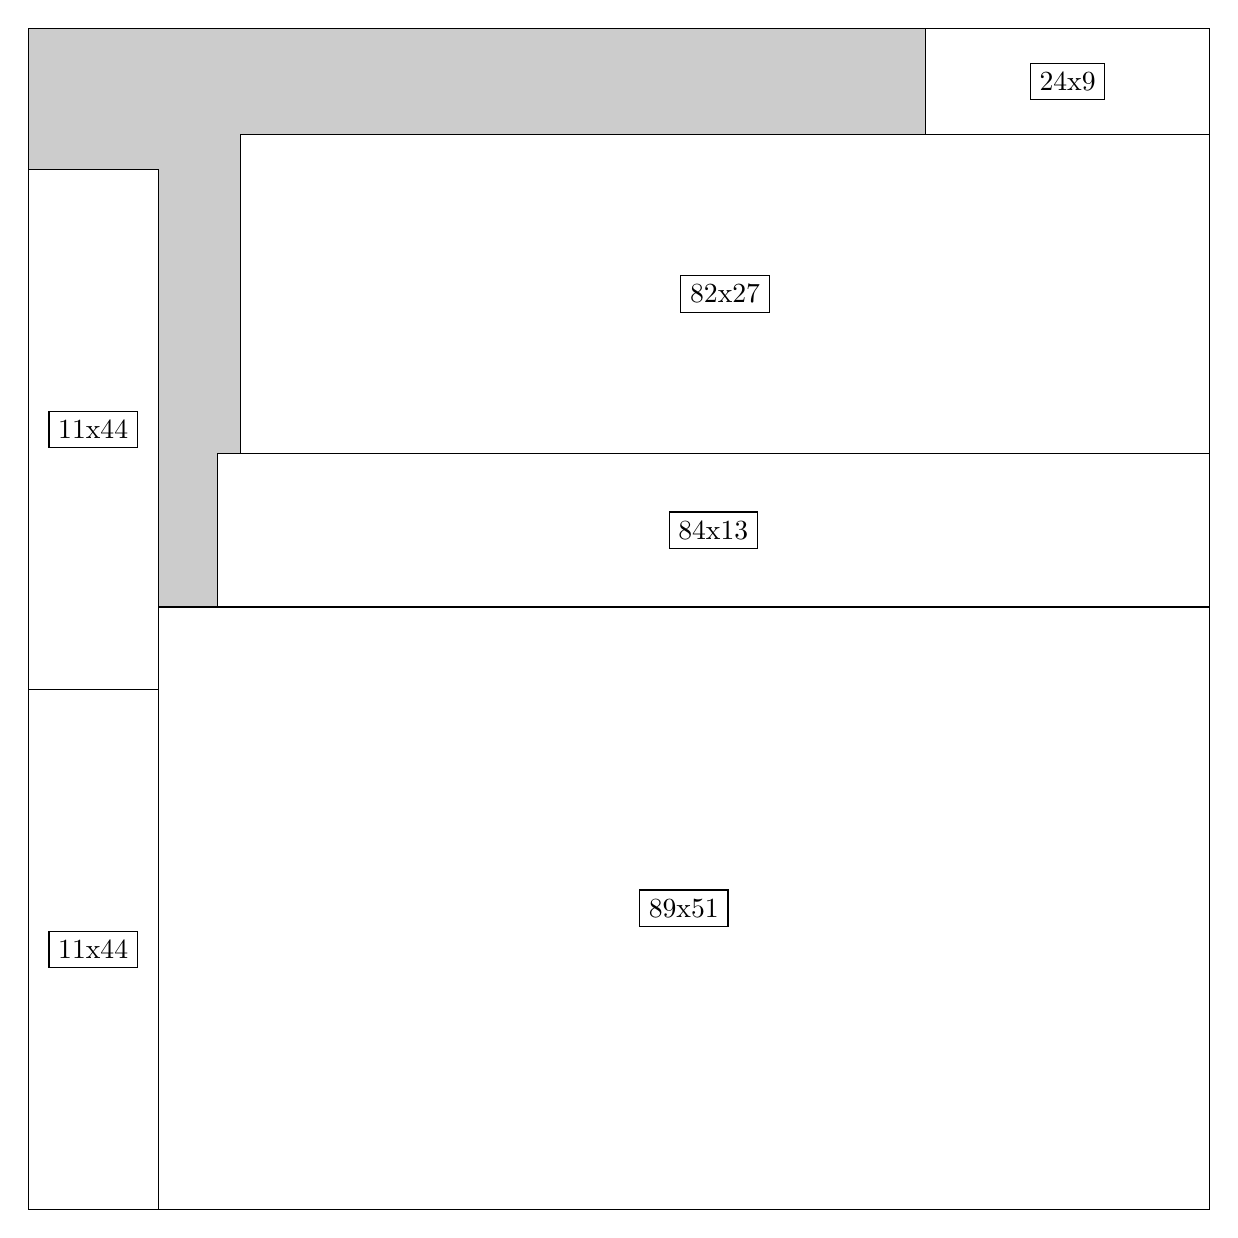
\begin{tikzpicture}[shorten >=1pt,scale=1.0,every node/.style={scale=1.0},->]
\tikzstyle{vertex}=[circle,fill=black!25,minimum size=14pt,inner sep=0pt]
\filldraw[fill=gray!40!white, draw=black] (0,0) rectangle (15.0,15.0);
\foreach \name/\x/\y/\w/\h in {89x51/1.65/0.0/13.35/7.6499999999999995,84x13/2.4/7.6499999999999995/12.6/1.95,82x27/2.6999999999999997/9.6/12.299999999999999/4.05,24x9/11.4/13.65/3.5999999999999996/1.3499999999999999,11x44/0.0/0.0/1.65/6.6,11x44/0.0/6.6/1.65/6.6}
\filldraw[fill=white!40!white, draw=black] (\x,\y) rectangle node[draw] (\name) {\name} ++(\w,\h);
\end{tikzpicture}


w =89 , h =51 , x =11 , y =0 , v =4539
\par
w =84 , h =13 , x =16 , y =51 , v =1092
\par
w =82 , h =27 , x =18 , y =64 , v =2214
\par
w =24 , h =9 , x =76 , y =91 , v =216
\par
w =11 , h =44 , x =0 , y =0 , v =484
\par
w =11 , h =44 , x =0 , y =44 , v =484
\par
\newpage


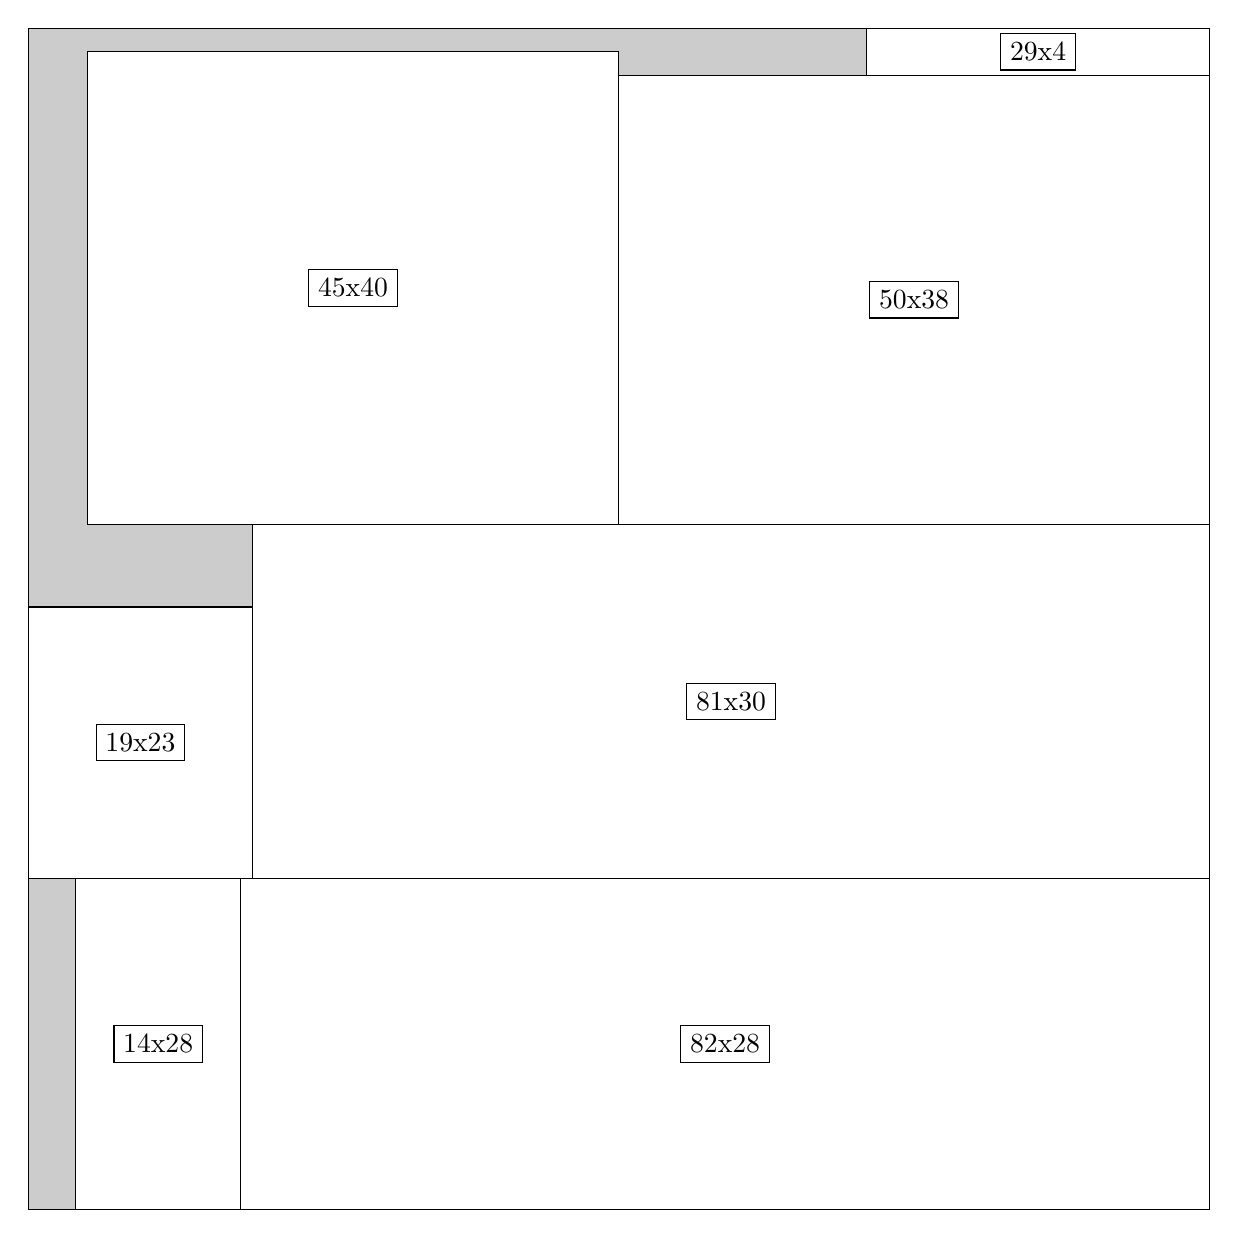
\begin{tikzpicture}[shorten >=1pt,scale=1.0,every node/.style={scale=1.0},->]
\tikzstyle{vertex}=[circle,fill=black!25,minimum size=14pt,inner sep=0pt]
\filldraw[fill=gray!40!white, draw=black] (0,0) rectangle (15.0,15.0);
\foreach \name/\x/\y/\w/\h in {82x28/2.6999999999999997/0.0/12.299999999999999/4.2,14x28/0.6/0.0/2.1/4.2,81x30/2.85/4.2/12.15/4.5,19x23/0.0/4.2/2.85/3.4499999999999997,50x38/7.5/8.7/7.5/5.7,29x4/10.65/14.399999999999999/4.35/0.6,45x40/0.75/8.7/6.75/6.0}
\filldraw[fill=white!40!white, draw=black] (\x,\y) rectangle node[draw] (\name) {\name} ++(\w,\h);
\end{tikzpicture}


w =82 , h =28 , x =18 , y =0 , v =2296
\par
w =14 , h =28 , x =4 , y =0 , v =392
\par
w =81 , h =30 , x =19 , y =28 , v =2430
\par
w =19 , h =23 , x =0 , y =28 , v =437
\par
w =50 , h =38 , x =50 , y =58 , v =1900
\par
w =29 , h =4 , x =71 , y =96 , v =116
\par
w =45 , h =40 , x =5 , y =58 , v =1800
\par
\newpage


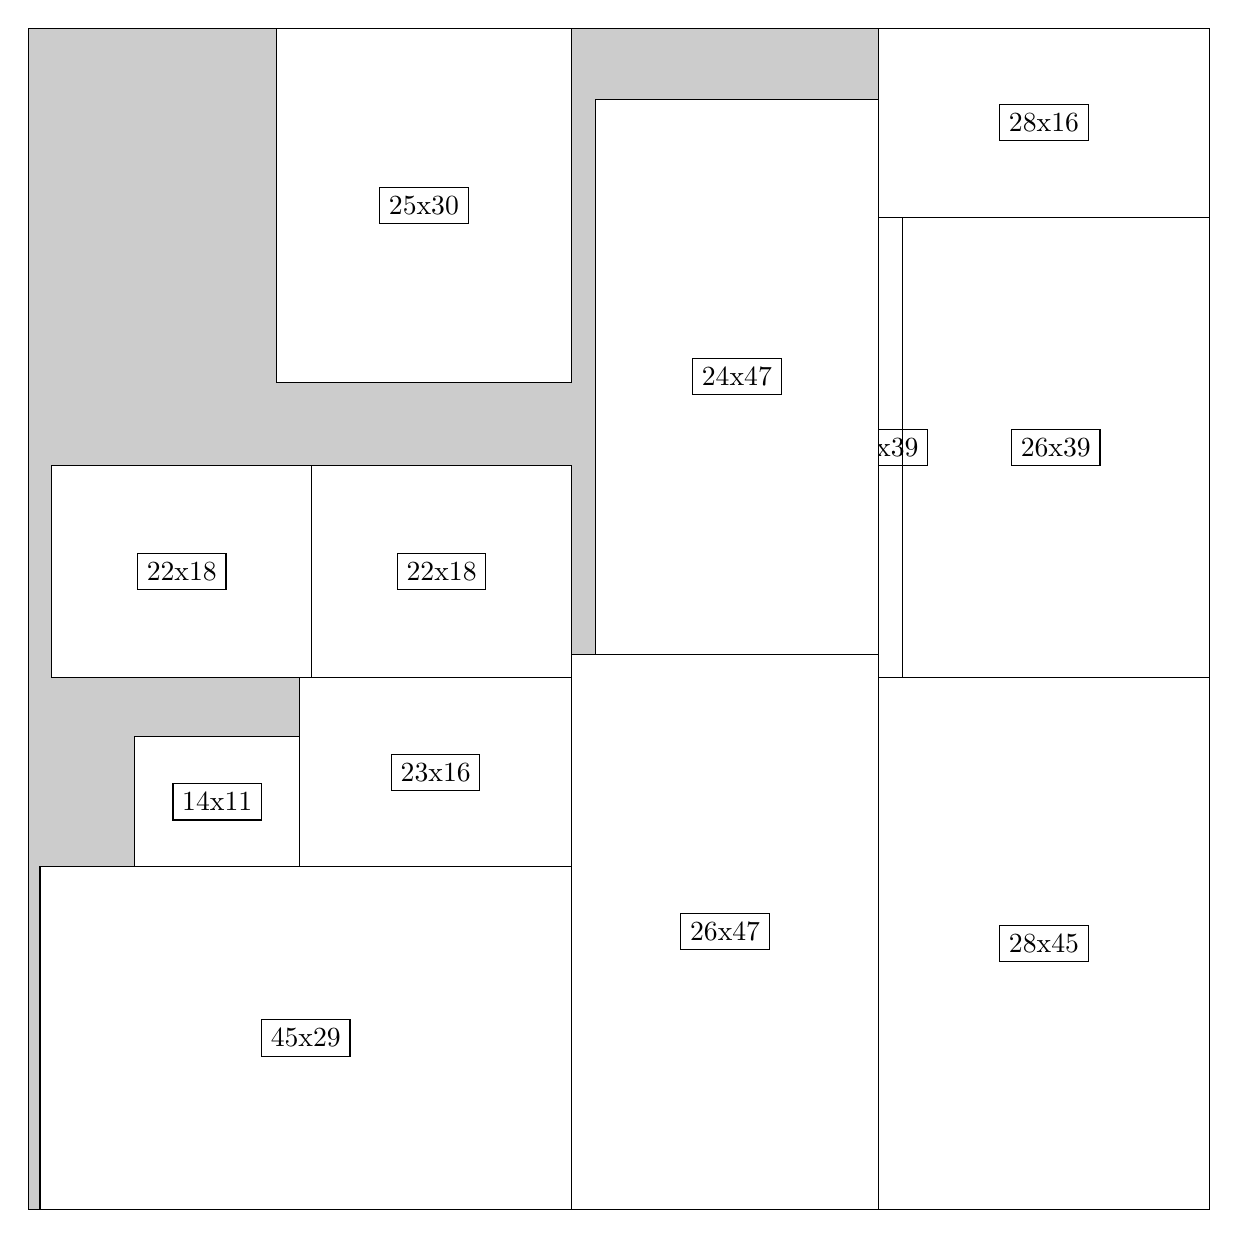
\begin{tikzpicture}[shorten >=1pt,scale=1.0,every node/.style={scale=1.0},->]
\tikzstyle{vertex}=[circle,fill=black!25,minimum size=14pt,inner sep=0pt]
\filldraw[fill=gray!40!white, draw=black] (0,0) rectangle (15.0,15.0);
\foreach \name/\x/\y/\w/\h in {28x45/10.799999999999999/0.0/4.2/6.75,26x39/11.1/6.75/3.9/5.85,2x39/10.799999999999999/6.75/0.3/5.85,28x16/10.799999999999999/12.6/4.2/2.4,26x47/6.8999999999999995/0.0/3.9/7.05,24x47/7.199999999999999/7.05/3.5999999999999996/7.05,45x29/0.15/0.0/6.75/4.35,23x16/3.4499999999999997/4.35/3.4499999999999997/2.4,14x11/1.3499999999999999/4.35/2.1/1.65,22x18/3.5999999999999996/6.75/3.3/2.6999999999999997,22x18/0.3/6.75/3.3/2.6999999999999997,25x30/3.15/10.5/3.75/4.5}
\filldraw[fill=white!40!white, draw=black] (\x,\y) rectangle node[draw] (\name) {\name} ++(\w,\h);
\end{tikzpicture}


w =28 , h =45 , x =72 , y =0 , v =1260
\par
w =26 , h =39 , x =74 , y =45 , v =1014
\par
w =2 , h =39 , x =72 , y =45 , v =78
\par
w =28 , h =16 , x =72 , y =84 , v =448
\par
w =26 , h =47 , x =46 , y =0 , v =1222
\par
w =24 , h =47 , x =48 , y =47 , v =1128
\par
w =45 , h =29 , x =1 , y =0 , v =1305
\par
w =23 , h =16 , x =23 , y =29 , v =368
\par
w =14 , h =11 , x =9 , y =29 , v =154
\par
w =22 , h =18 , x =24 , y =45 , v =396
\par
w =22 , h =18 , x =2 , y =45 , v =396
\par
w =25 , h =30 , x =21 , y =70 , v =750
\par
\newpage


\end{document}